\subsection{Группы номенклатуры}
\subsubsection{Описание изменений ,,Группы номенклатуры``}
%\marginnote{\Date{Вт.}{07}{Апр.}{2017}}[-40pt]
\begin{itemize}	
	\item В конфигурацию добавлено новое перечисление содержащее названия групп номенклатуры <<A,B,C>> 
	\item Изменения в справочнике ,,Номенклатура``.\par
	В справочник ,,Номенклатура`` на закладку ,,Учетная информация`` добавлен новый реквизит ,,Группы номенклатуры`` Рис.~\ref{ris:1.jpg}	
	\begin{figure}[H]
		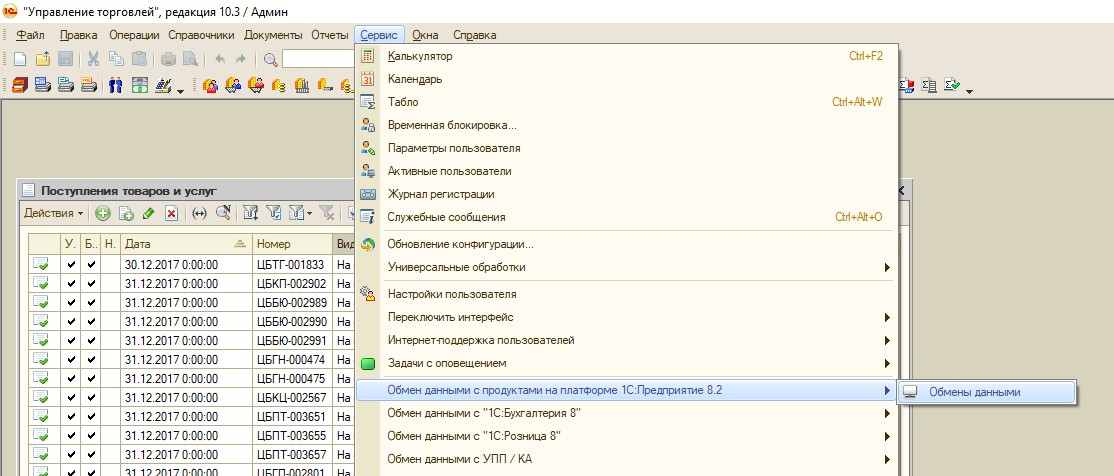
\includegraphics[width=0.8\textwidth]{1.jpg}
		\caption{Добавлен реквизит.}
		\label{ris:1.jpg}
	\end{figure}
   Существует возможность заполнить \index{entry} реквизит одним из трех значений хранящихся в перечислении Рис.~\ref{ris:2.jpg}	
	\begin{figure}[H]
		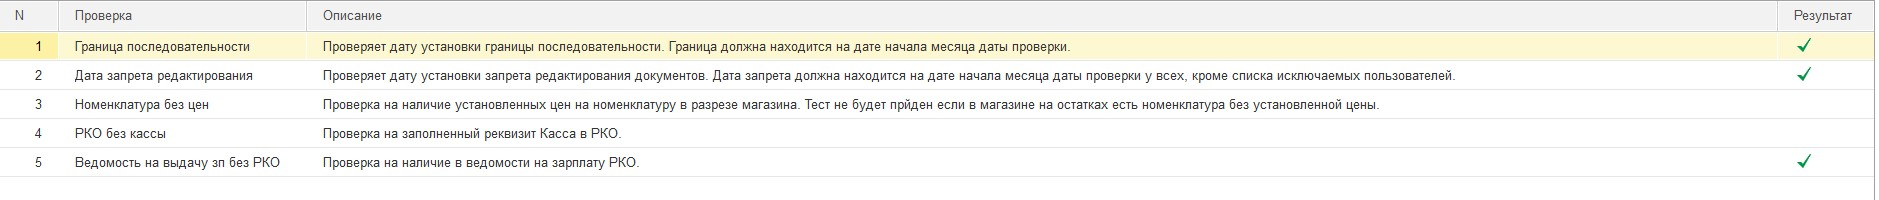
\includegraphics[width=0.8\textwidth]{2.jpg}
		\caption{Выбор значения.}
		\label{ris:2.jpg}
	\end{figure}
	Выбрав нужное значение нужно воспользоваться кнопкой 
	
\includegraphics[width=0.02\linewidth]{images/sv} ,,Записать``  или \keys{Записать закрыть}  для сохранения изменений Рис.~\ref{ris:3.jpg}
	\begin{figure}[H]
		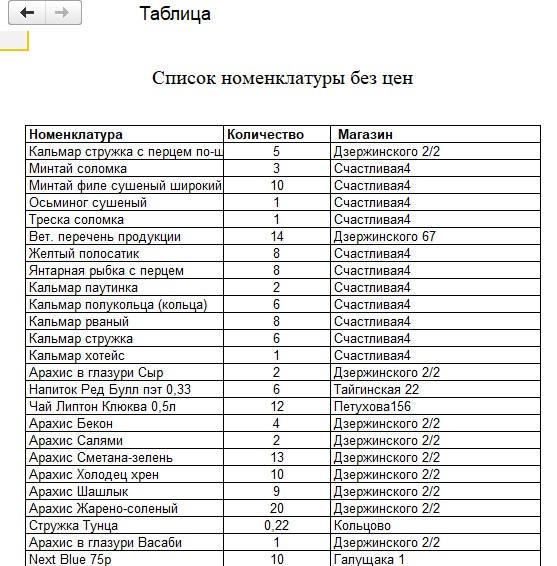
\includegraphics[width=0.8\textwidth]{3.jpg}
		\caption{Сохранить изменения.}
		\label{ris:3.jpg}
	\end{figure}
	\item После того как в элементы номенклатуры были добавлены значения  ,,Групп номенклатуры`` появляется возможность формирования отчетов с их использованием
\end{itemize}

\subsubsection{Формирование отчетов с использованием ,,Группы номенклатуры``}
	Формирование отчета будет рассмотрено на примере отчета ,,Оценка валовой прибыли``. Отчет находится в разделе \menu[,]{Продажи, Отчеты по продажам, Показатели эффективности, ...}
	
\begin{itemize}	

	\item Открываем отчет
	\item Выбираем \keys{Настройки}  Рис.~\ref{ris:4.jpg}	
	\begin{figure}[H]
		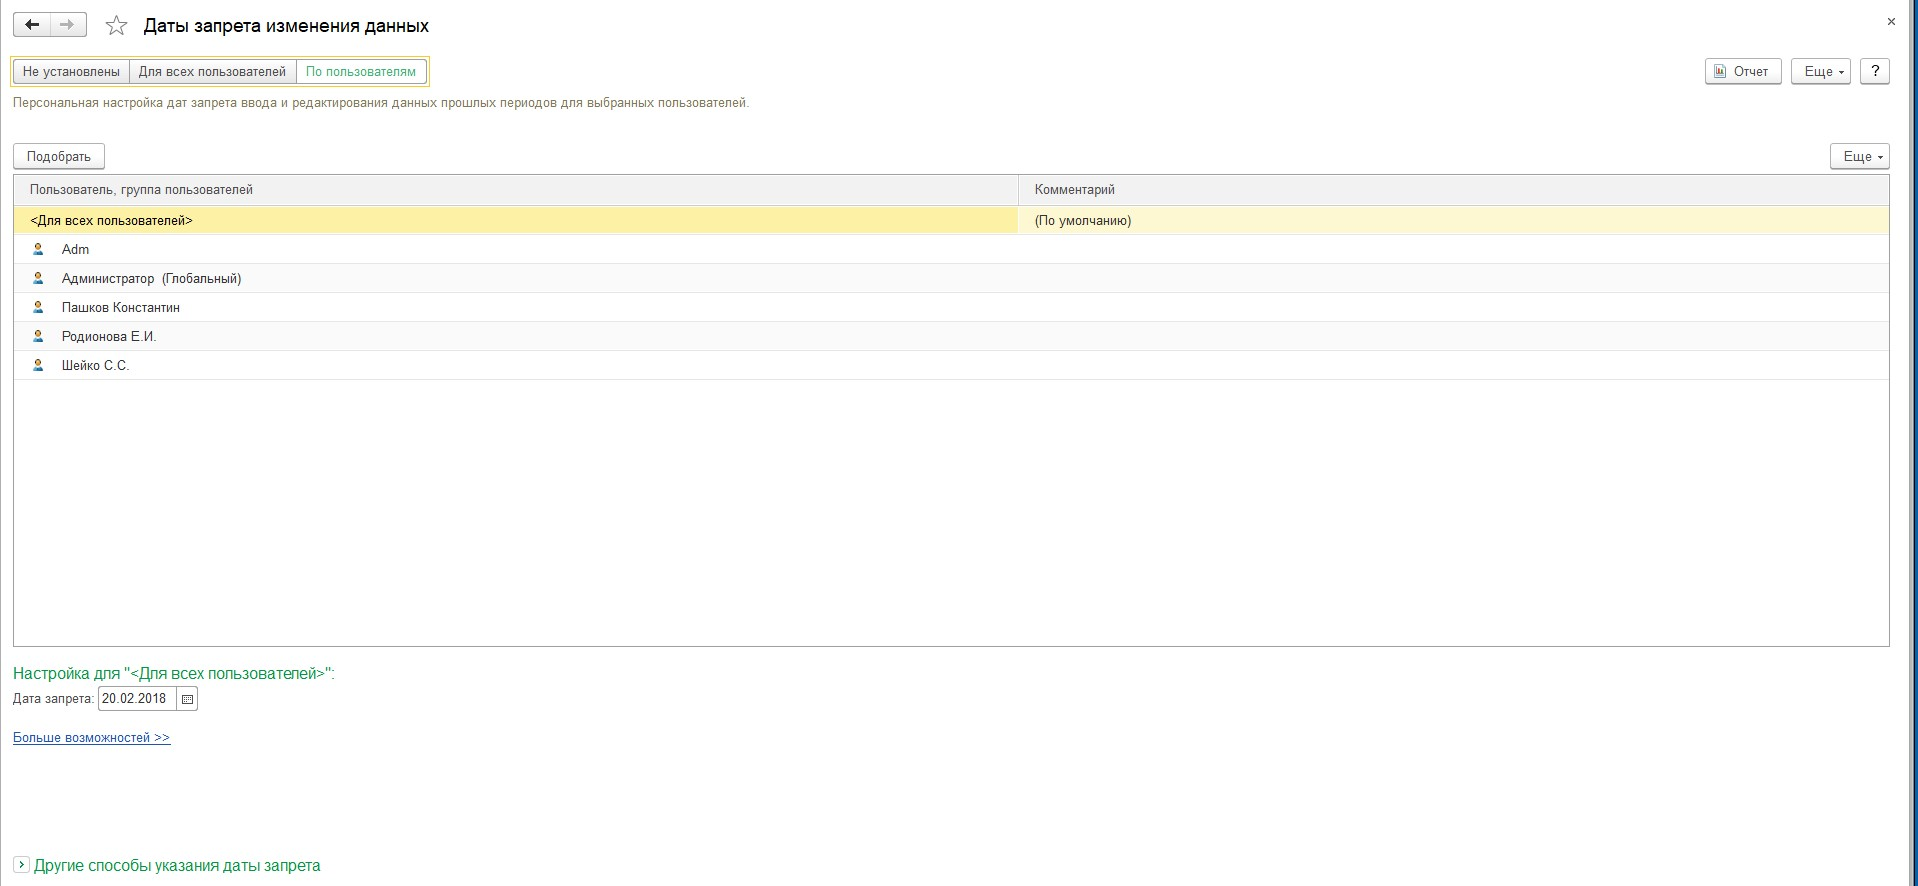
\includegraphics[width=0.8\textwidth]{4.jpg}
		\caption{Открыть настройки.}
		\label{ris:4.jpg}
	\end{figure}
	\item	В открывшейся форме настроек нужно нажать кнопку \keys{Расширенный}  Рис.~\ref{ris:5.jpg}
	 Рис.~\ref{ris:2.jpg}	
	\begin{figure}[H]
		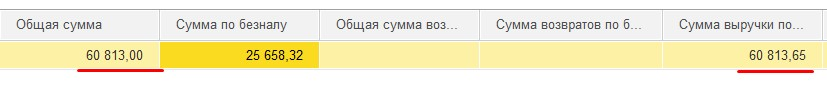
\includegraphics[width=0.8\textwidth]{5.jpg}
		\caption{Расширенные настройки.}
		\label{ris:5.jpg}
	\end{figure} 
	\item	Теперь нам нужно добавить отбор по новому реквизиту, для этого нажмите кнопку \keys{Добавить отбор}
 Рис.~\ref{ris:6.jpg}
	\begin{figure}[H]
		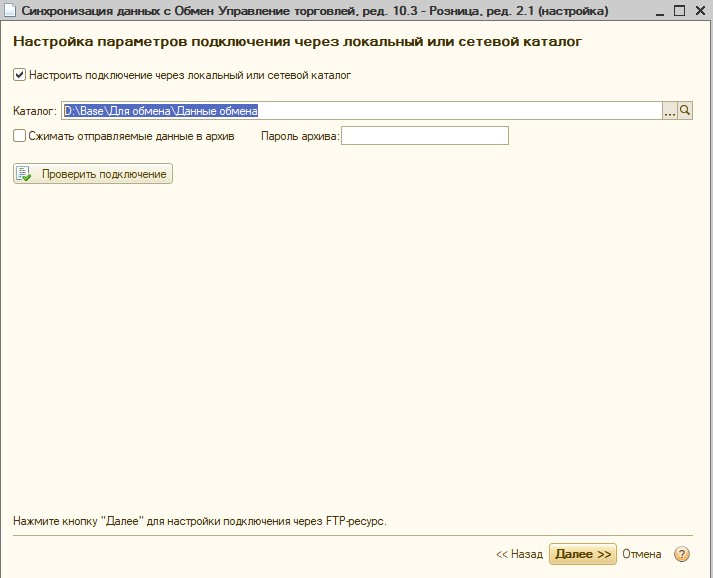
\includegraphics[width=0.8\textwidth]{6.jpg}
		\caption{Добавить отбор.}
		\label{ris:6.jpg}
	\end{figure}



	\item В открывшемся окне ,,Выбор поля отчета`` кликнув на крестике рядом со строчкой ,,Номенклатуры``,
	развернем эту ветку для выбора нужного реквизита Рис.~\ref{ris:7.jpg}	
\begin{figure}[H]
	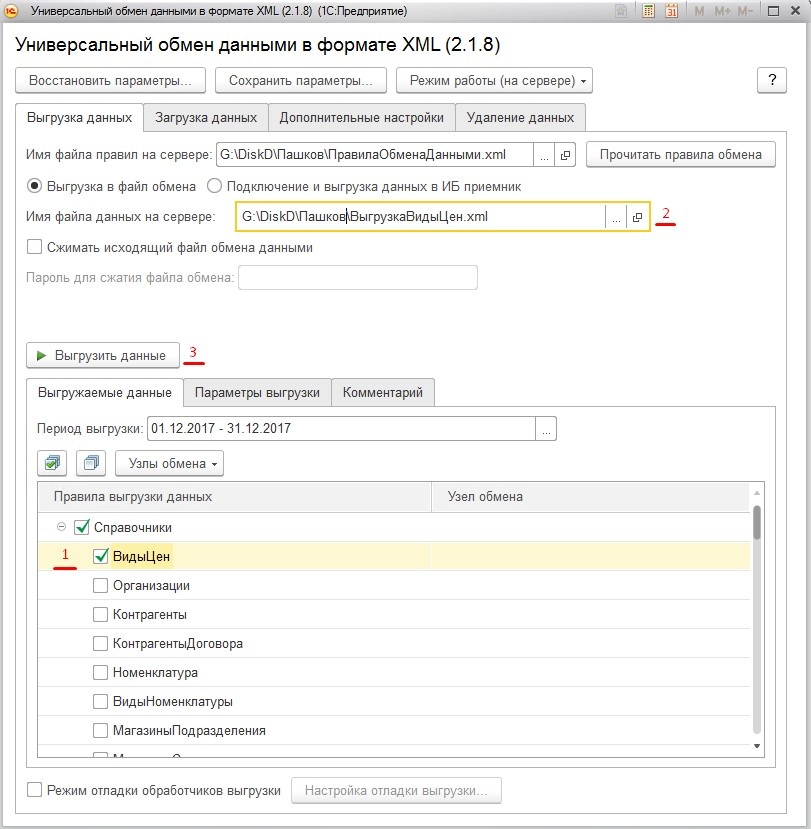
\includegraphics[width=0.8\textwidth]{7.jpg}
	\caption{Номенклатура.}
	\label{ris:7.jpg}
\end{figure}
	\item	Двойным кликом мыши выбираем  ,,Группа Номенклатуры`` Рис.~\ref{ris:8.jpg}
Рис.~\ref{ris:2.jpg}	
\begin{figure}[H]
	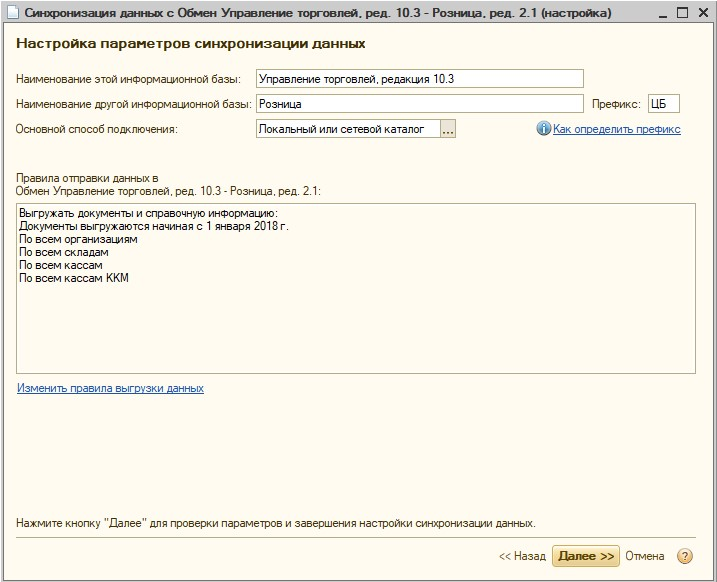
\includegraphics[width=0.8\textwidth]{8.jpg}
	\caption{Выбор реквизита.}
	\label{ris:8.jpg}
\end{figure} 
\item Теперь ,,Группа номенклатуры`` добавлена в поля отбора, кликнув в соответствующей строке на поле 
,,Значение`` нужно выбрать нужное нам значение ,,Группы номенклатуры``.
Рис.~\ref{ris:9.jpg}
\begin{figure}[H]
	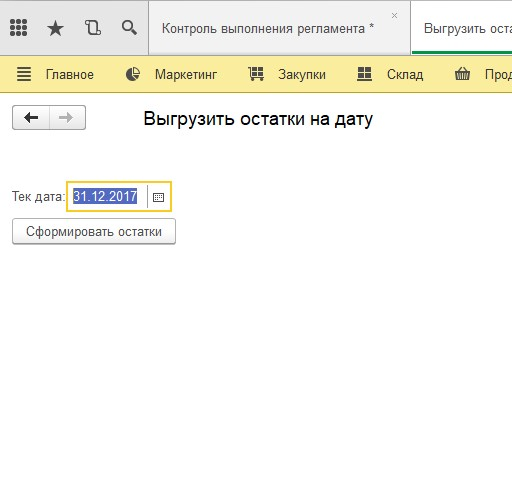
\includegraphics[width=0.8\textwidth]{9.jpg}
	\caption{Выбор группы.}
	\label{ris:9.jpg}
\end{figure}

\item Для удобства использования добавим выбранную группировку в шапку отчета. Для этого нужно дважды кликнуть мышкой в соответствующей строке на колонке со  ,,звездочкой`` и выбрать ,,В шапке отчета``
Рис.~\ref{ris:10.jpg}
\begin{figure}[H]
	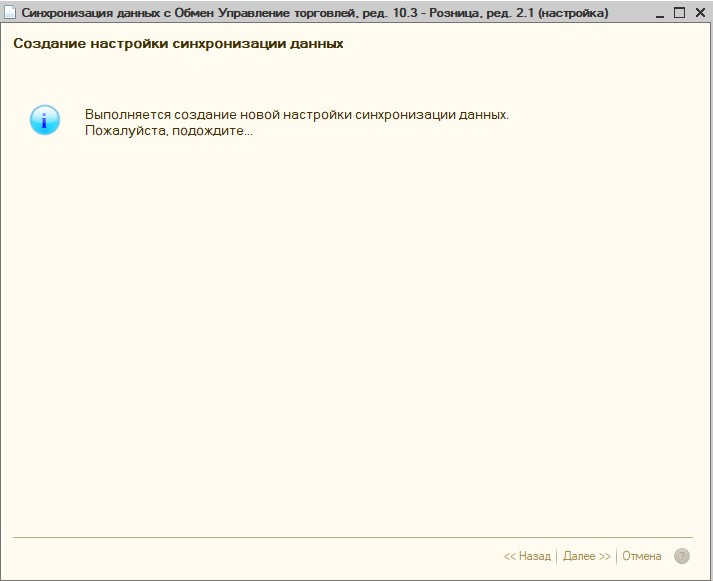
\includegraphics[width=0.8\textwidth]{10.jpg}
	\caption{Фиксировать в шапке.}
	\label{ris:10.jpg}
\end{figure}


\item Теперь форма настроек выглядит примерно следующим образом Рис.~\ref{ris:11.jpg}
\begin{figure}[H]
	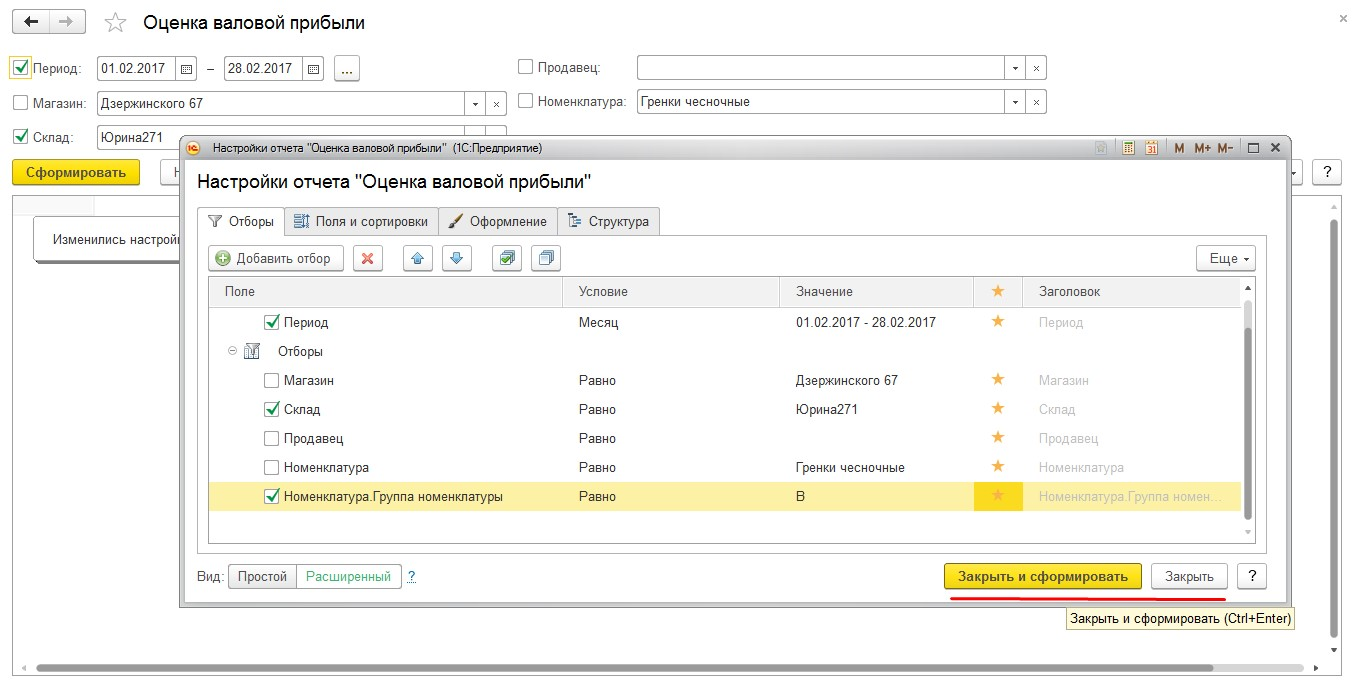
\includegraphics[width=0.8\textwidth]{11.jpg}
	\caption{Настроенные группировки.}
	\label{ris:11.jpg}
\end{figure}
Для сохранения изменений можно воспользоваться кнопками \keys{Закрыть и сформировать} или  \keys{Закрыть}.
В первом случае сразу после закрытия формы начнется формирование отчета, во-втором просто закроется форма настроек.

\item В шапке отчета появился отбор по нужному реквизиту. Рис.~\ref{ris:12.jpg}
\begin{figure}[H]
	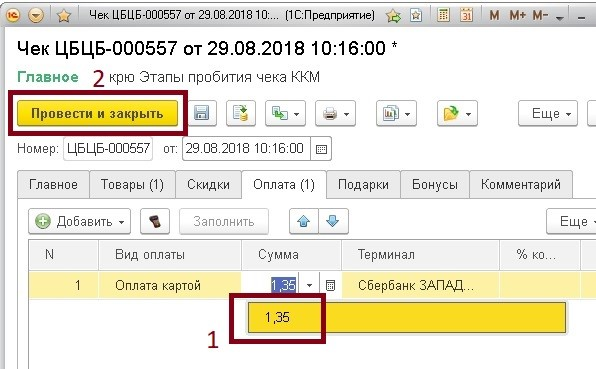
\includegraphics[width=0.8\textwidth]{12.jpg}
	\caption{Настроенный отчет.}
	\label{ris:12.jpg}
\end{figure}

Можно формировать отчет.
	
\end{itemize}
